
\section{Containerization with Singularity}

\begin{figure}[h]
    \begin{center}
    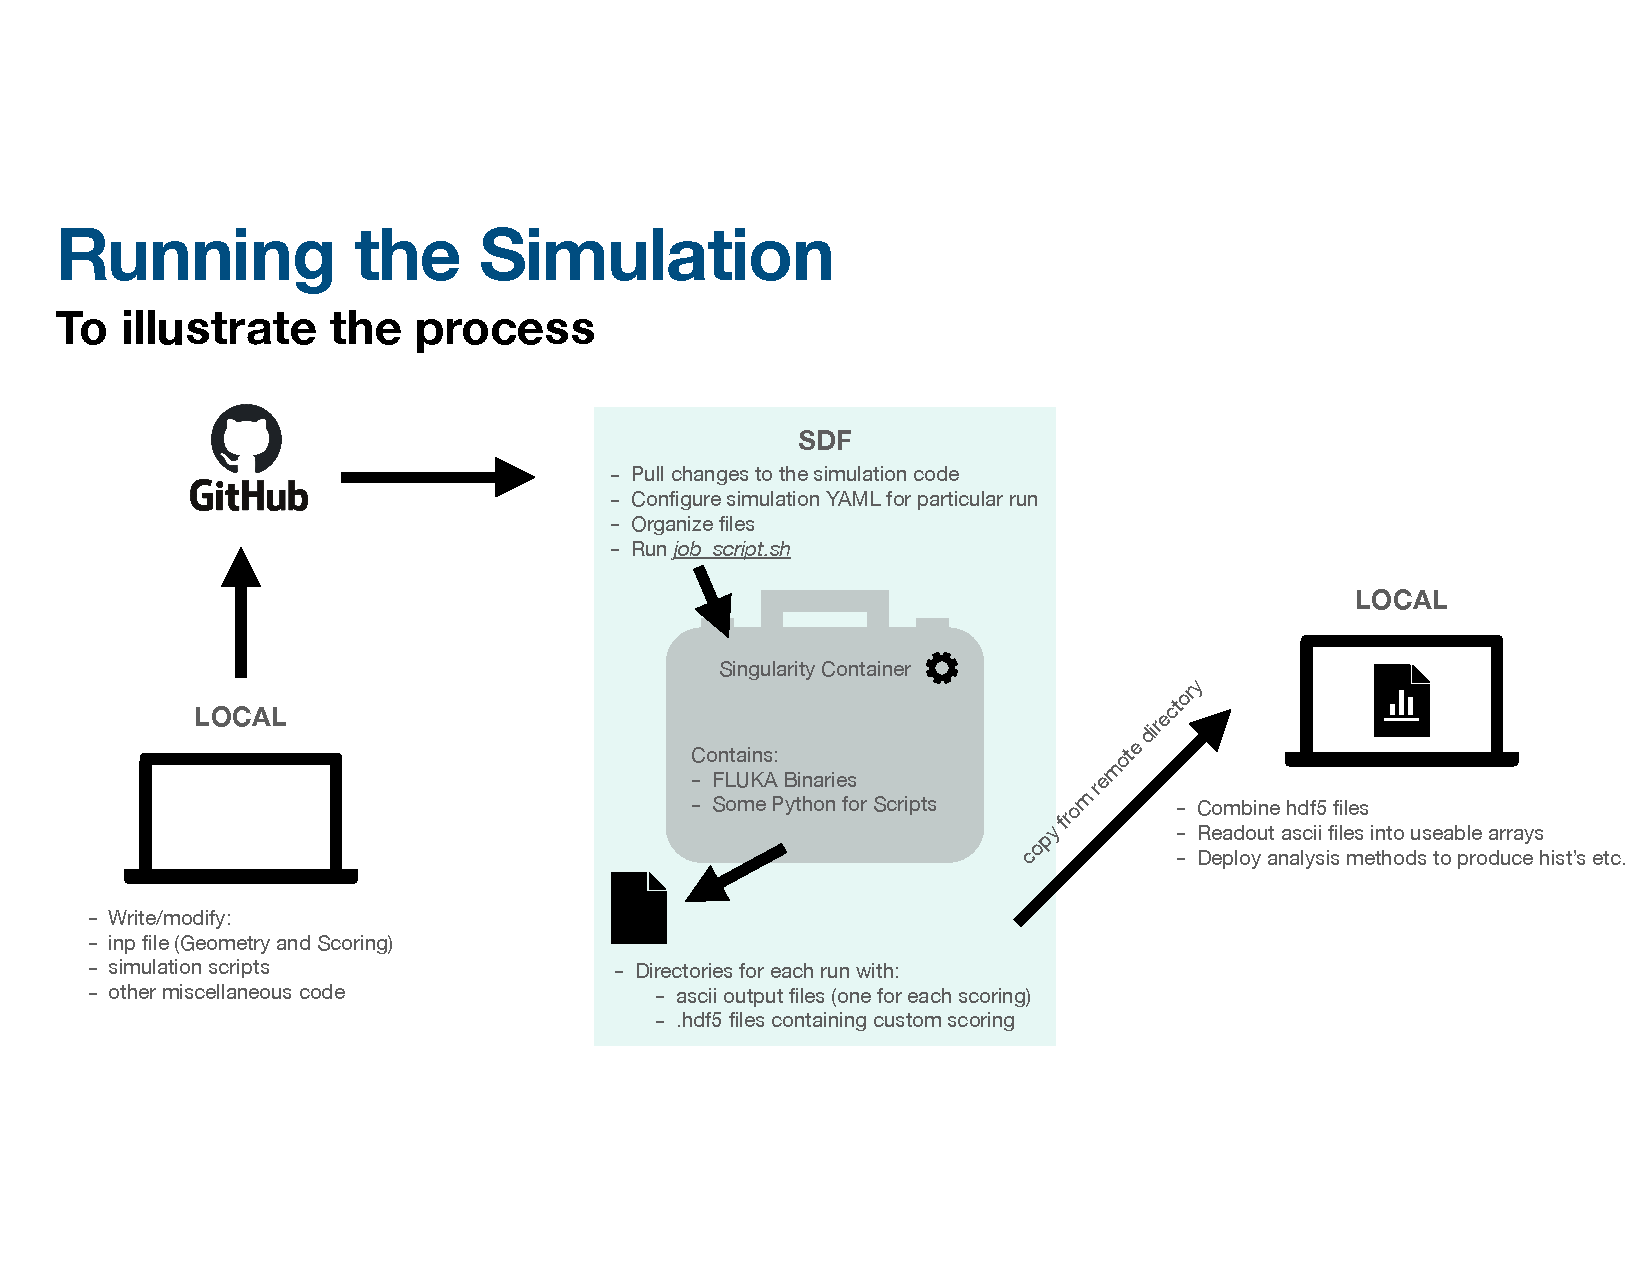
\includegraphics[scale=0.5]{figures/sim_diagram.pdf}
    \caption{A visualization of the remote simulation and development process}
    \label{fig:process1}
    \end{center}
\end{figure}

\paragraph{}
In order to deploy FLUKA on a remote cluster, SDF for instance, it must be packaged up in a \textit{container}. SDF recommends using Singularity which is essentially designed for containerizing software with its dependencies to maximize portability. Naturally, there are a few caveats to containerizing the simulation. The first, rather inconvenient constraint is that Singularity containers must (at the time of writing) be built from within a Linux OS. Therefore, to build a Singularity image using a Mac, one must use a linux VM. This requires, among other pieces, Vagrant which is used to run the Linux virtual machine. There's no use in giving a comprehensive guide to installing Singularity, Vagrant and creating the entire Singularity image here; these softwares are actively being developed and improved. Readers are referred to the Sylabs Singularity documentation: \url{https://docs.sylabs.io/guides/3.11/admin-guide/installation.html#mac}.

\paragraph{}
The definition file ``\begin{tt}.def\end{tt}'' for the Singularity container is in the Github repository. Should the reader wish to reproduce or modify the container, they'll need at minimum a CERN FLUKA licence in order to download the FLUKA binaries and they'll need to be placed in the directory where the container will be created along with any other files and software that cannot be installed separately from within the ``\begin{tt}.def\end{tt}'' file.

\paragraph{}
Put simply, the Singularity container holds some Python packages, the FLUKA binaries and an Evaluated Nuclear Data File (ENDF) database holding cross sections read by FLUKA when transporting neutrons.